\documentclass[hyperref=unicode,graphics=pdflatex,13pt]{beamer}
\usepackage[utf8]{inputenc}
\usepackage[T2A]{fontenc}
\usepackage[english,russian]{babel}
\usepackage{color, colortbl}
\usepackage{tabularx}
\usepackage{graphicx}
\usepackage{subfigure}
\usepackage[
    backend=biber,
    bibencoding=utf8,
    autolang=other
]{biblatex}
\renewbibmacro{in:}{}
\addbibresource{presentation.bib}
\mode<presentation>
{
  \usetheme{Madrid}
  \setbeamercovered{invisible}
  \setbeamertemplate{footline}{\hfill\large{\insertframenumber/\inserttotalframenumber}~~}
  \setbeamersize{text margin left=0.4cm,sidebar width left=0cm}
}

\graphicspath{{picture/}, {template/}, {tests/}}

\usepackage{tikz}
\usetikzlibrary{arrows}
\usepackage{forest}

\newcommand{\ttwo}{fill=black!40}
\newcommand{\tthr}{fill=black!70}

\beamertemplatenavigationsymbolsempty
\DeclareGraphicsRule{.1}{mps}{*}{}

\usepackage{etoolbox}

\setbeamertemplate{theorems}[numbered] 
\undef{\lemma}
\undef{\corollary}
\newtheorem{lemma}{Лемма}
\newtheorem{corollary}{Следствие}

\newcommand\highlight[1]{{\color{blue}{#1}}}
\newcommand\col[1]{{\color{olivegreen}{#1}}}

\title{Разработка эффективной структуры данных, поддерживающей инкрементальные изменения, для параллельной обработки деревьев}
\author[У Цзюньфэн]{Автор: У Цзюньфэн, группа M4236\\Научный руководитель: Станкевич А.С.\\Консультант: Буздалов М.В}
\institute[Университет ИТМО]{ Кафедра компьютерных технологий \\Факультет ИТиП \\
\includegraphics[height=.3\textheight]{template/itmo_small_white_rus.jpg}}
\date[20.06.2016]{20 июня 2016 года}

\begin{document}

\begin{frame}[noframenumbering,plain,shrink]
  \titlepage
\end{frame}

\begin{frame}[shrink]{Мотивация: Структуры данных для динамических деревьев}
    \begin{itemize}
        \item Структура данных поддерживает лес (укорененных) деревьев
        \begin{itemize}
            \item на вершинах могут быть пометки
            \item на ребрах могут быть пометки
        \end{itemize}
        \item Операции модификации:
        \begin{itemize}
            \item добавление вершины
            \item подвешивание вершины в качестве ребенка другой вершины
            \item отцепление вершины от ее родителя
        \end{itemize}
        \item Запросы:
        \begin{itemize}
            \item корень дерева, в котором находится данная вершина
            \item правда ли, что две вершины в одной компоненте связности
            \item сумма вершинных пометок в поддереве данной вершины
            \item сумма реберных пометок на пути между двумя вершинами
        \end{itemize}
        \item Зачем?
        \begin{itemize}
            \item эффективные алгоритмы поиска максимального потока
            \item \ldots
        \end{itemize}
    \end{itemize}
\end{frame}

\begin{frame}[shrink]{Цель и задачи}
\begin{itemize}
\item Цель исследования
\begin{itemize}
\item Разработка структуры данных на основе Rake-and-Compress деревьев для параллельной обработки деревьев, поддерживающей инкрементальные изменения: добавление нового узла, подвешивание узла в 
качестве ребенка другого узла, отцепление узла от его родителя, изменение меток на вершинах и ребрах.
 \end{itemize}
\end{itemize}

\begin{itemize} \item Задачи
\begin{enumerate}
    \item снятие ограничения на число детей вершины, присущее параллельным реализациям Rake-and-Compress деревьев;
    \item уменьшение использования памяти с $\Theta(n \log n)$ до $\Theta(n)$, где $n$~--- общее число вершин в деревьях, при сохранении эффективности параллельных операций;
    \item обеспечение поддержки меток произвольных типов для вершин и ребер, при условии что метки на вершинах являются элементами коммутативного моноида, а метки на ребрах~---
          элементами произвольного моноида.
\end{enumerate}
\end{itemize}
\end{frame}

\begin{frame}[shrink]{Техническое задание и исходные данные к работе}
\begin{itemize}
\item Требуется разработать структуру данных для параллельной обработки деревьев, поддерживающую инкрементальные изменения. 
\item В разработанной структуре данных требуется снять ограничение на максимальную степень вершины, имеющееся у существующих реализаций.
\item Требуется поддержка эффективного выполнения запросов на определения корня дерева по представителю дерева, определение групповой суммы меток в поддереве данной вершины и на пути между двумя данными вершинами. 
\item Структуру данных требуется реализовать на языке C++ с использованием библиотеки PASL для реализации параллельных операций.
\end{itemize}
\end{frame}

\begin{frame}[shrink]{Rake-and-Compress Tree}
\begin{itemize}
    \item Исходное дерево подвергается одновременному применению операций Rake и Compress для всех 
          возможных вершин
\end{itemize}
\centering
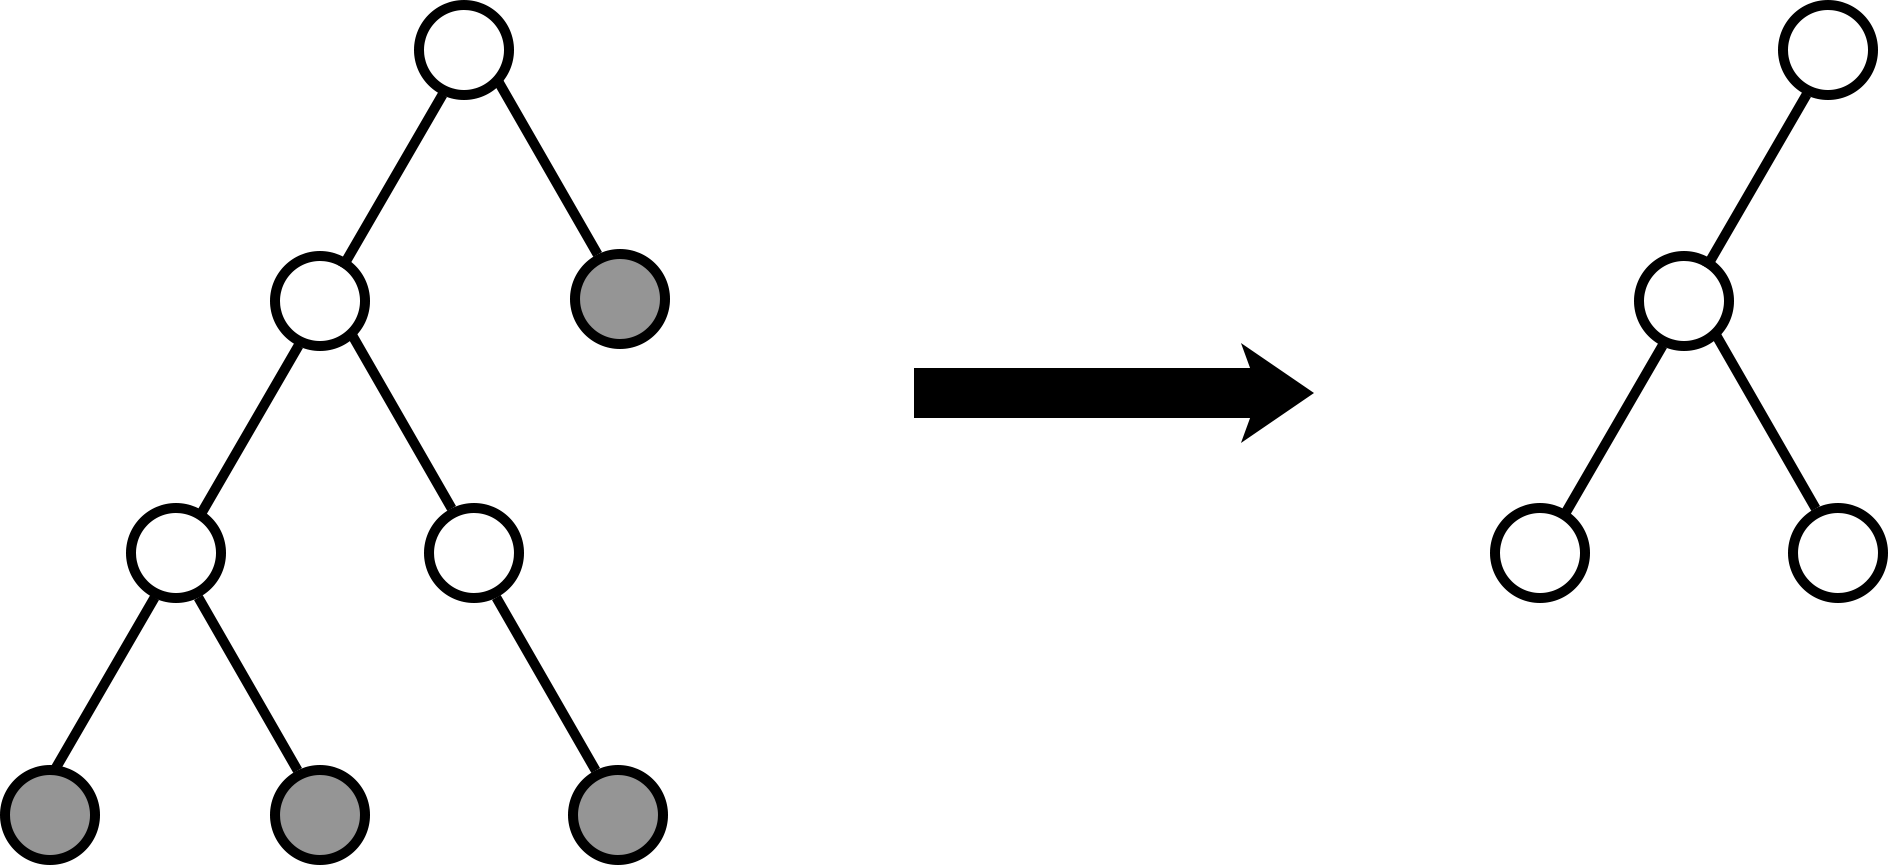
\includegraphics[width=0.4\textwidth]{picture/rake.png}~~~~~~~
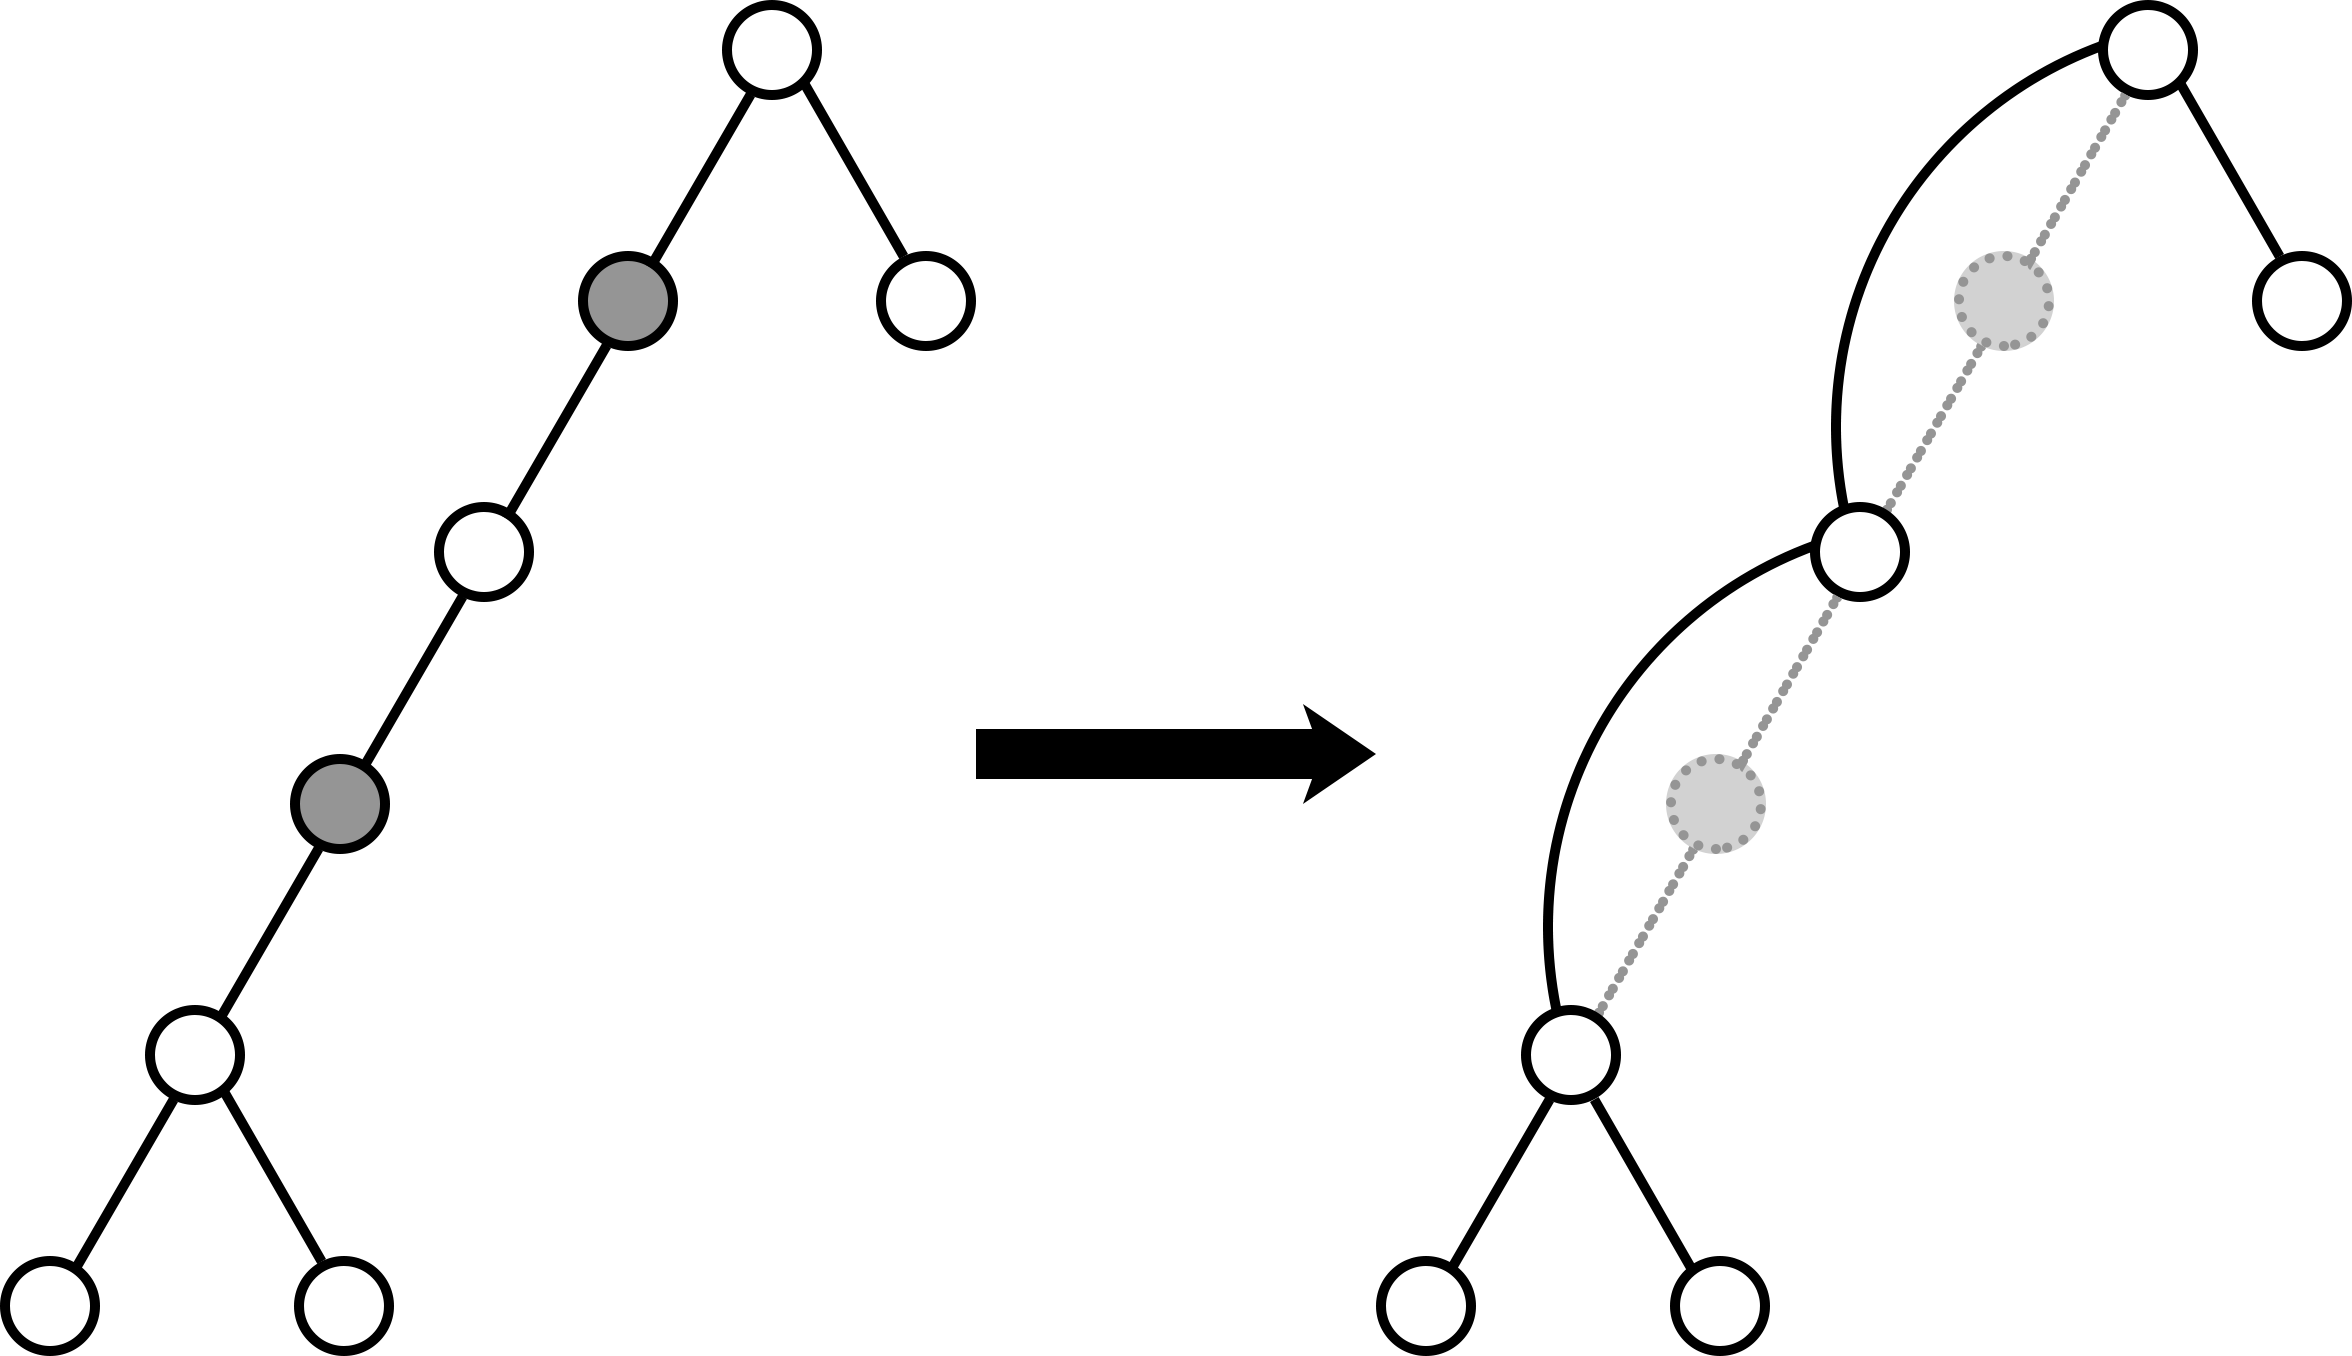
\includegraphics[width=0.4\textwidth]{picture/compress.png}
\begin{itemize}
    \item Применяем эту процедуру к дереву, пока оно не сожмется в одну вершину
    \item $O(\log n)$ уровней, каждый уровень~--- различная степень подробности представления 
          дерева
\end{itemize}
\end{frame}

\begin{frame}[shrink]{Rake-and-Compress Tree: Общая картина}
\centering
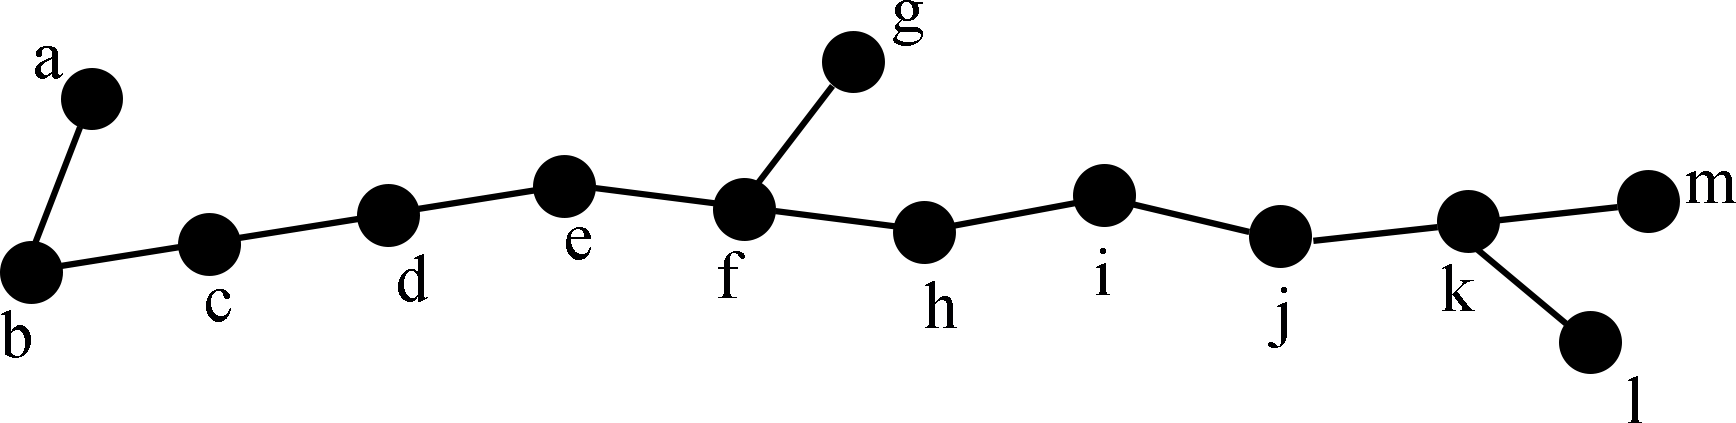
\includegraphics[width=0.7\textwidth]{picture/rc_tree_1_primitive_tree.png}\\

\includegraphics[width=0.9\textwidth]{picture/rc_tree_2_completed_clustering.png}
\end{frame}

\begin{frame}[shrink]{Преимущества и недостатки RC-деревьев}
\begin{itemize}
        \item Преимущества
	\begin{itemize}
    		\item Поддерживает запросы на поддеревьях и на путях
		\item Может строиться параллельно
		\item Поддерживает произвольные модификации
		\item Может применять пакеты обновлений параллельно
	\end{itemize}
\end{itemize}
\begin{itemize}
        \item Недостатки
	\begin{itemize}
	    \item Эффективно работает, только если число детей вершины ограничено константой
	    \item Сложная реализация с разбором большого числа случаев
	    \item Параллелизм $\to$ проблемы с памятью $\to$ $\Theta(n \log n)$ памяти в простой реализации
	    \item Переиспользуемых реализаций пока нет
	\end{itemize}
\end{itemize}
\end{frame}

\begin{frame}[shrink]{Предлагаемая реализация (1/2)}
\begin{itemize}
    \item Снятие ограничений на степень вершины~--- разделение каждой вершины на вершину данных и вершину связей,
          организация детей в декартово дерево
\end{itemize}
\begin{center}
\scalebox{0.7}{
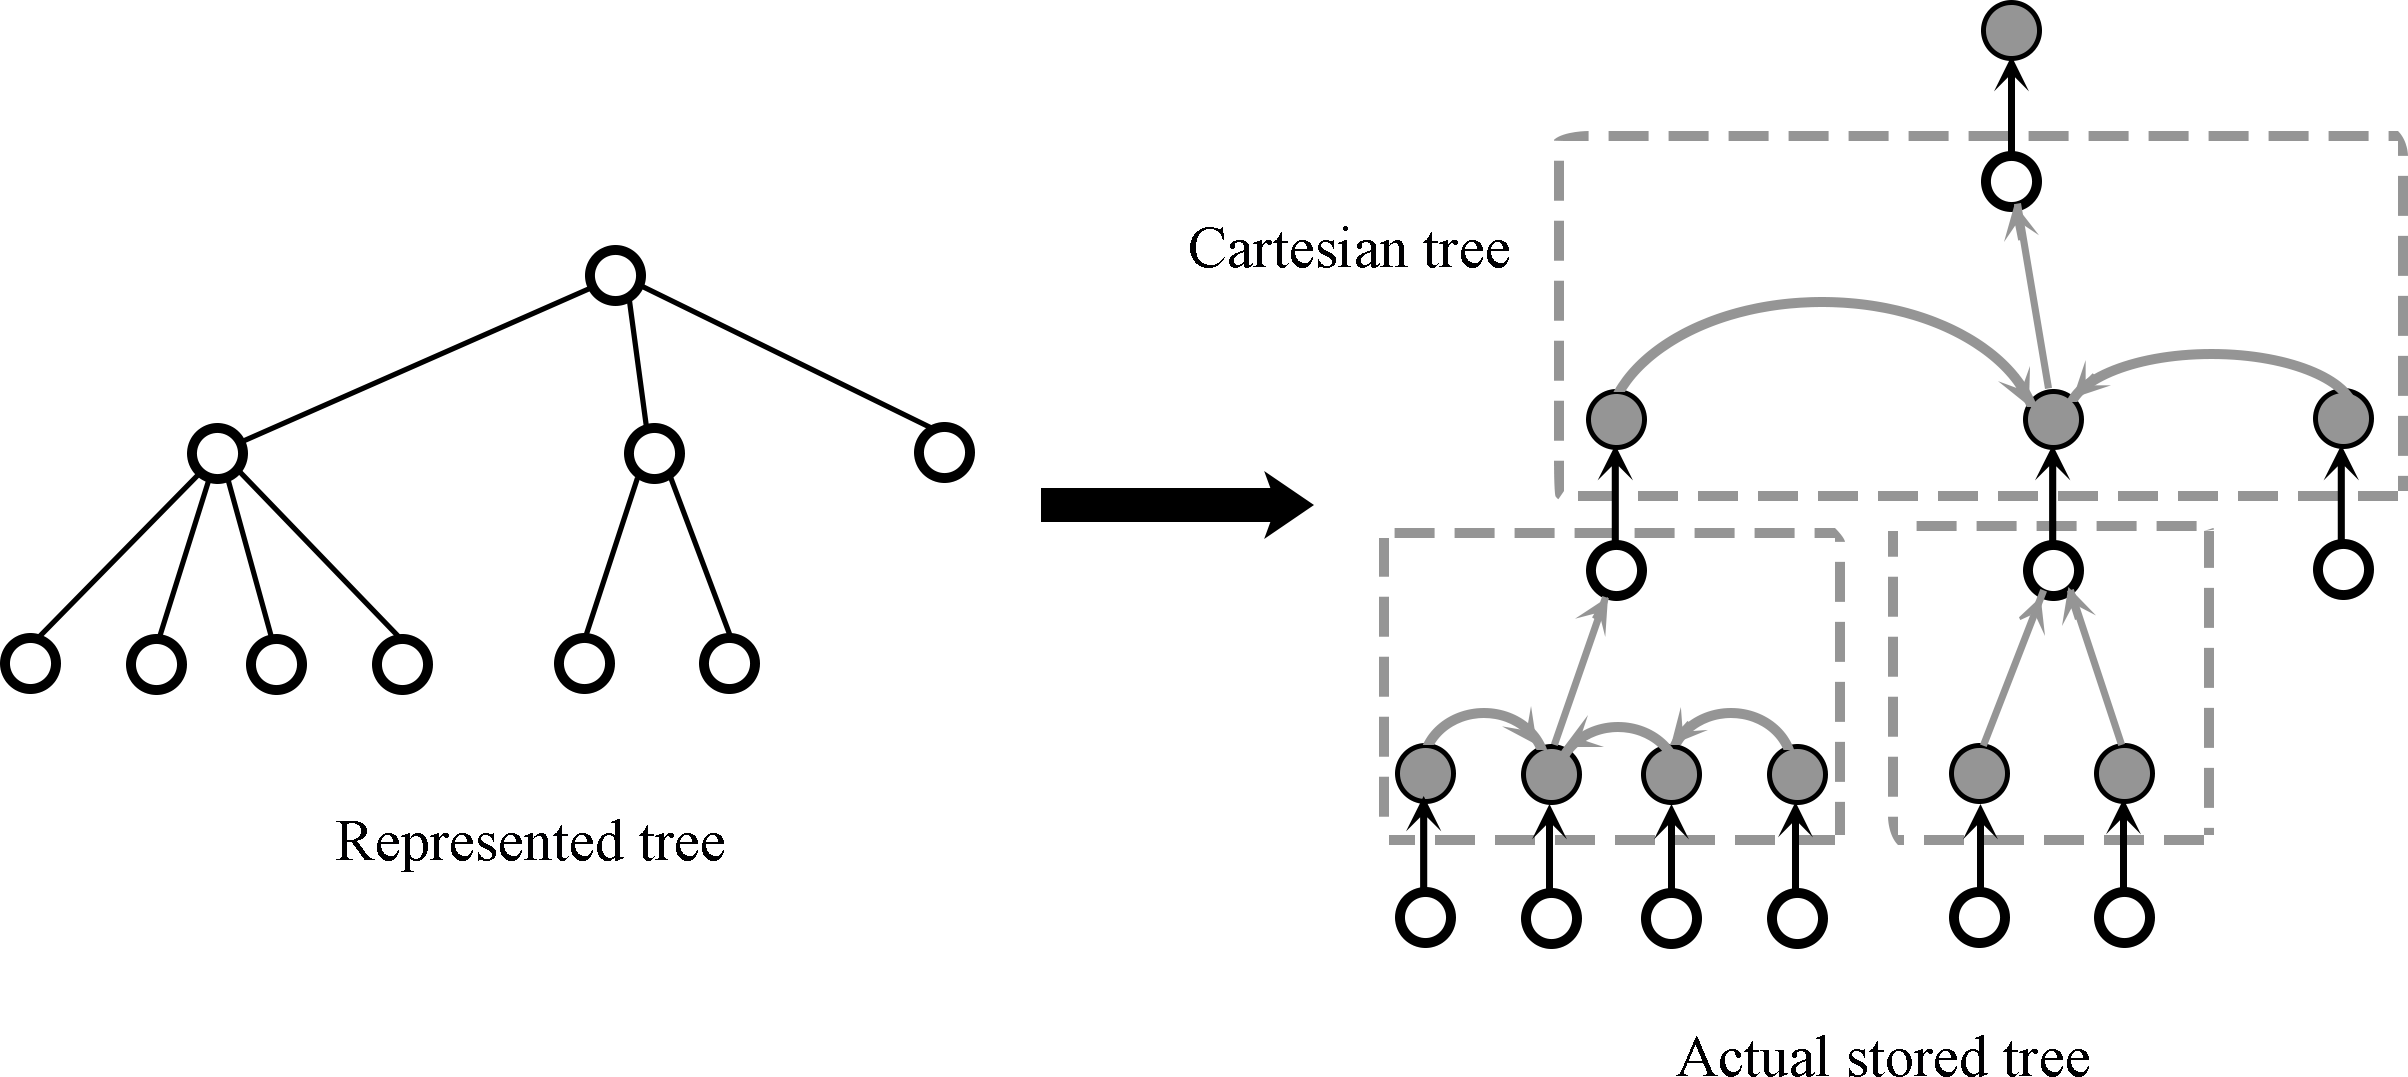
\includegraphics[width=0.9\textwidth]{picture/represented_tree_and_actual_stored_tree.png}}
\end{center}
\begin{itemize}
    \item Пометки на вершинах~--- элементы коммутативного моноида, на ребрах~--- элементы 
          произвольного моноида
    \begin{itemize}
        \item Вершины связей имеют нулевые пометки на вершинах и ребрах~--- результаты запросов
              не зависят от структуры
    \end{itemize}
\end{itemize}
\end{frame}

\begin{frame}[shrink]{Предлагаемая реализация (2/2)}
\begin{itemize}
    \item Решение проблем с памятью~--- вектор <<живых>> инкарнаций вершин для каждой вершины
    \item Для четных и нечетных слоев~--- разные векторы для разделения чтения слоя $i$ и записи слоя $i+1$
\end{itemize}
\begin{center}
\scalebox{0.75}{
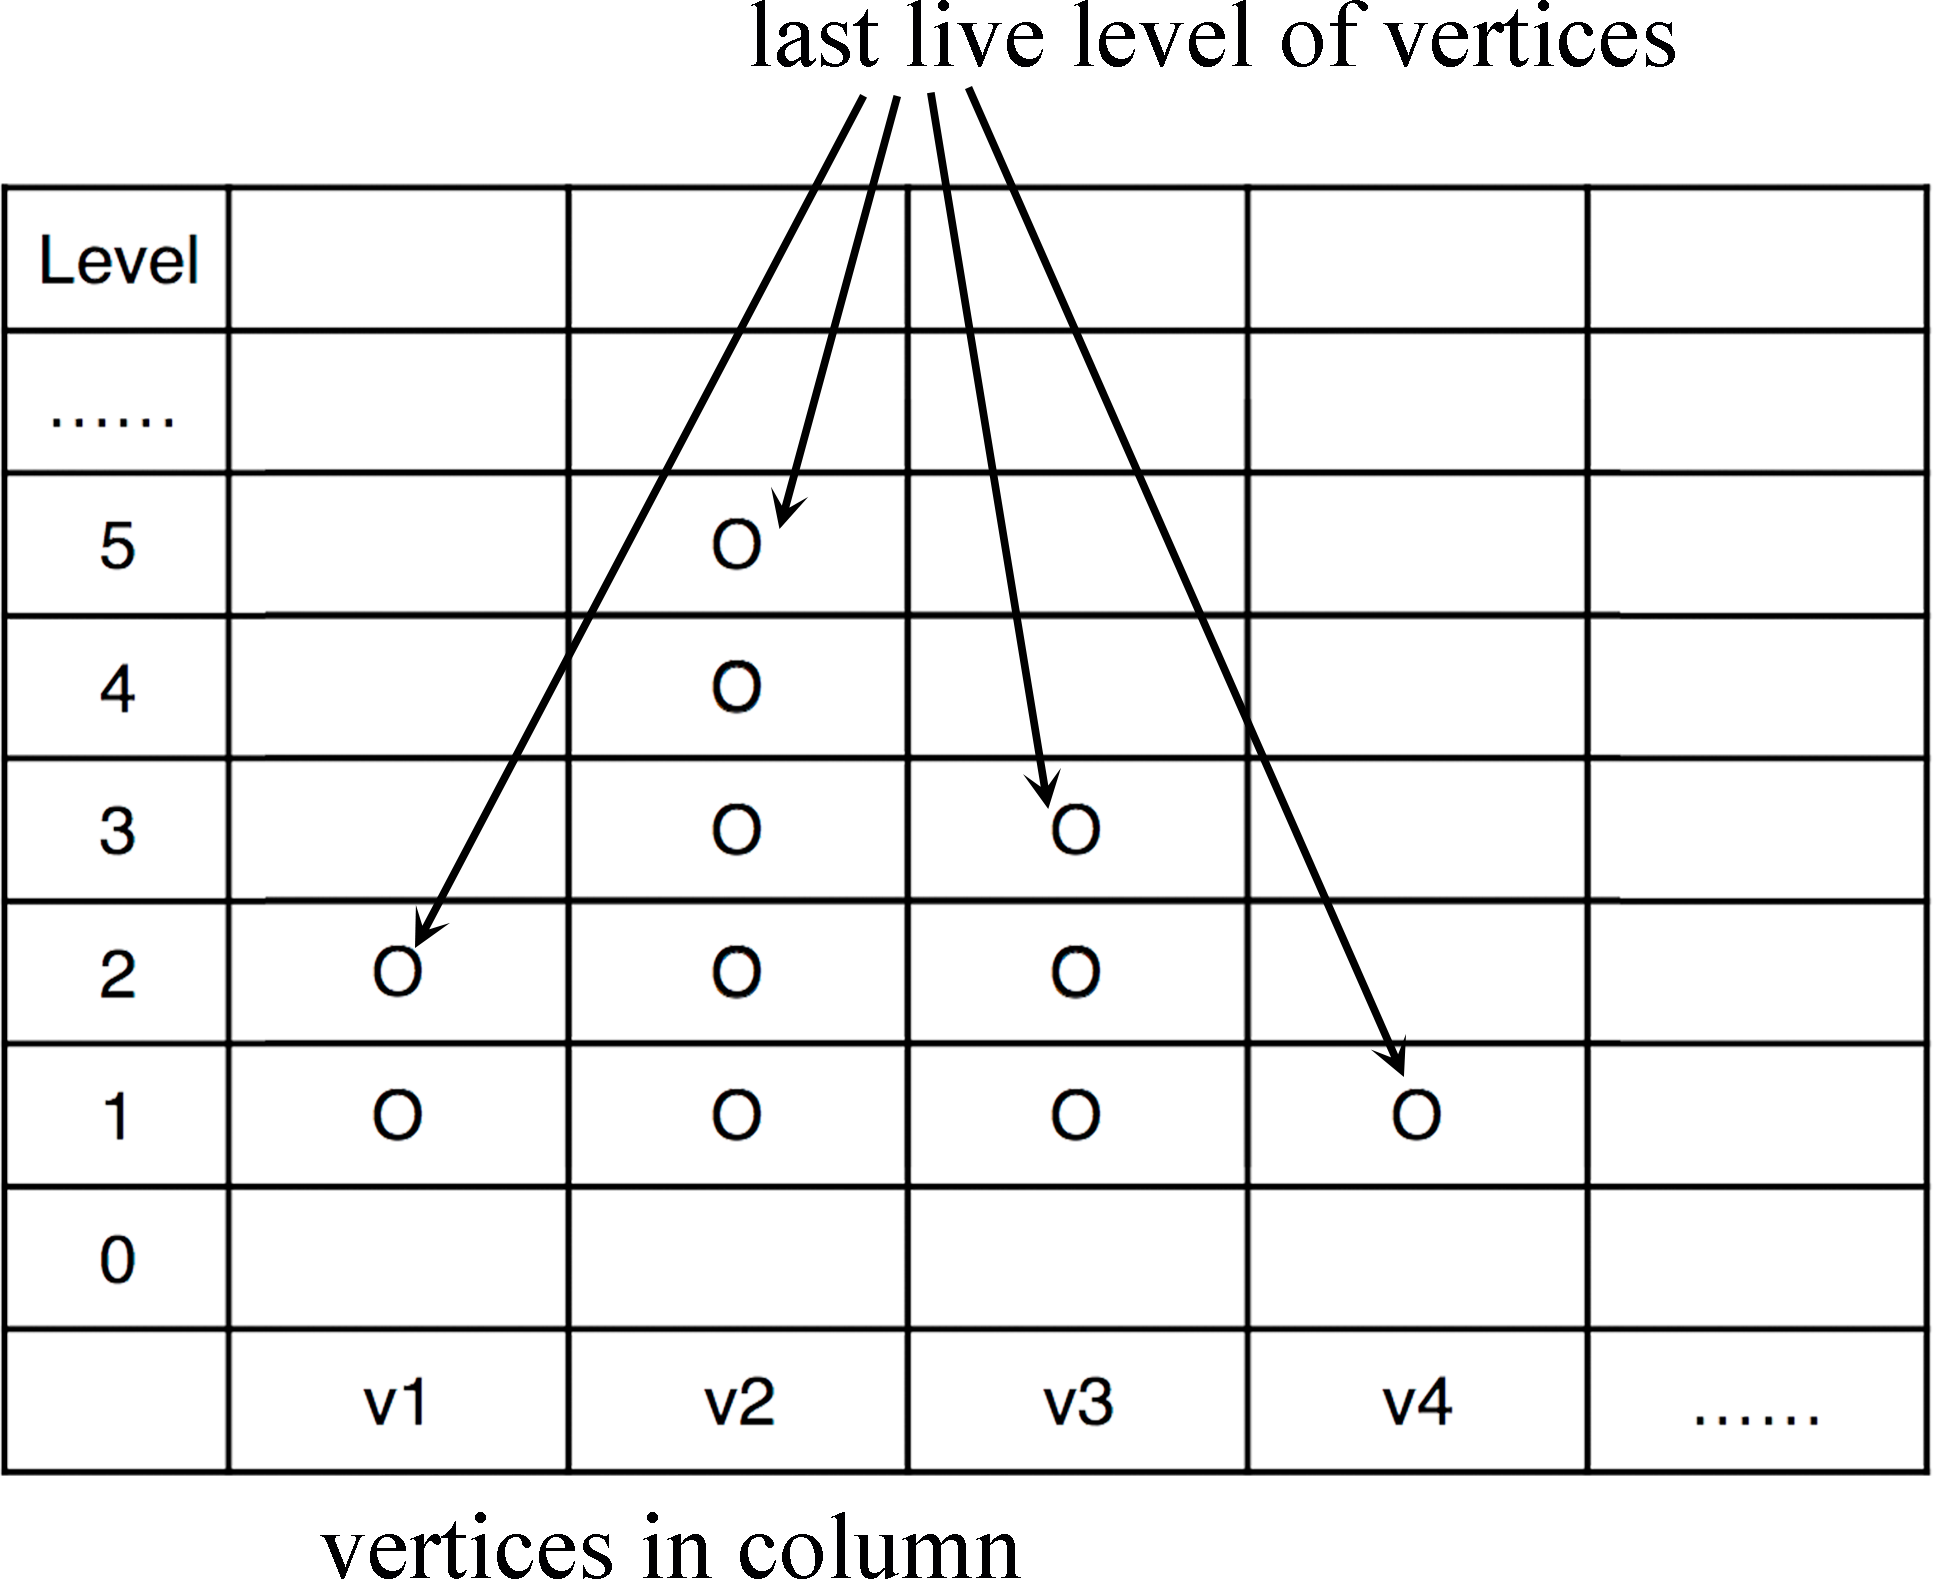
\includegraphics[width=0.6\textwidth]{picture/vertices_in_column.png}}
\end{center}
\end{frame}

\begin{frame}[shrink]{Распараллеливание}
\begin{itemize}
    \item В алгоритме используется две распараллеливаемые операции
        \begin{itemize}
            \item Цикл FOR
            \item Вычисление префиксных сумм:
                  \\~~~~даны числа $x_{1}, x_{2}, ..., x_{n}$
                  \\~~~~вычислить $s_{1}=x_{1}, s_{2}=x_{1}+x_{2}, ..., s_{n}=x_{1}+x_{2}+...+x_{n}$
        \end{itemize}
    \item Реализации операций
        \begin{itemize}
            \item Последовательная (Sequential)
            \item Параллельная с использованием OpenMP
            \item Параллельная с использованием PASL
        \end{itemize}
\end{itemize}
\end{frame}

\begin{frame}[shrink]{Результаты эксперимента}
\begin{itemize}
    \item Тесты:
	\begin{enumerate}
	    \item Дерево-<<палка>>: $n$ вершин, при этом $i$-тая вершина является ребенком $(i-1)$-ой 
	вершины при $i > 0$
	    \item Дерево-<<пучок>>: $n$ вершин, при этом $i$-тая вершина является ребенком вершины 0 при 
	$i > 0$
	    \item Дерево-<<два пучка>>: $n$ вершин при $n = 2m$, $m$ целое, при этом вершина 0 является 
	родителем вершин с 1 по $(m-1)$, 
	вершина $m$ является родителем вершин с $(m+1)$ по $(n-1)$, а вершины 0 и $m$ 
	дополнительно соединены
	    \item Построение дерева-<<палки>> в десять этапов, каждый из которых состоит в присоединении 
	$n / 10$ вершин
	\end{enumerate}
    \item Тестовый сервер: восемь ядер, Intel Xeon E5606, 2.13 ГГц
    \item Следующие слайды: время работы на тестах в секундах
\end{itemize}
\end{frame}

\begin{frame}[shrink]{Результаты экспериментов: одно ядро}

\begin{table}[!ht]
\centering
\scalebox{0.75}{
\begin{tabular}{|l|l|l|l|l|}\hline
Sequential	& $n=10000$ & $n=100000$ & $n=1000000$ & $n=3000000$ \\\hline
1 long chain & 0.063533	& 0.936087 & 9.8946 & 31.3906 \\\hline
2 large degree & 0.031963 & 0.473844 & 5.04014 & 16.8301 \\\hline
3 two large degrees & 0.03333 & 0.495401 & 5.19158 & 16.8656 \\\hline
4 incremental long chain & 0.068615 & 0.840358 & 11.1828 & 36.3289 \\\hline
\end{tabular}}
\end{table}

\begin{table}[!ht]
\centering
\scalebox{0.75}{
\begin{tabular}{|l|l|l|l|l|}\hline
OpenMP	& $n=10000$ & $n=100000$ & $n=1000000$ & $n=3000000$ \\\hline
1 long chain & 0.07072 & 1.01285 & 11.4329 & 35.1043 \\\hline
2 large degree & 0.033578 & 0.48801 & 5.46487 & 17.5146 \\\hline
3 two large degrees & 0.035731 & 0.515872 & 5.68942 & 18.0354 \\\hline
4 incremental long chain & 0.075208 & 0.891592 & 12.389 & 40.6775 \\\hline
\end{tabular}}
\end{table}

\begin{table}[!ht]
\centering
\scalebox{0.75}{
\begin{tabular}{|l|l|l|l|l|}\hline
PASL	& $n=10000$ & $n=100000$ & $n=1000000$ & $n=3000000$ \\\hline
1 long chain & 0.073684	& 1.09323 & 12.3956 & 38.1296 \\\hline
2 large degree & 0.036832 & 0.522955 & 5.75152 & 18.5603 \\\hline
3 two large degrees & 0.038104 & 0.548474 & 6.03994 & 19.1851 \\\hline
4 incremental long chain & 0.078299 & 0.953348 & 13.0366 & 42.883 \\\hline
\end{tabular}}
\end{table}
\end{frame}

\begin{frame}[shrink]{Результаты экспериментов: одно ядро}
\begin{center}
\begin{figure}
\centering
\scalebox{0.65}{
\subfigure{      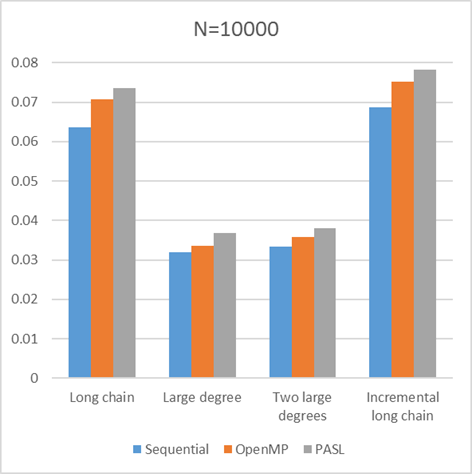
\includegraphics[width=0.45\textwidth]{tests/results-1-a.png} }
\subfigure{      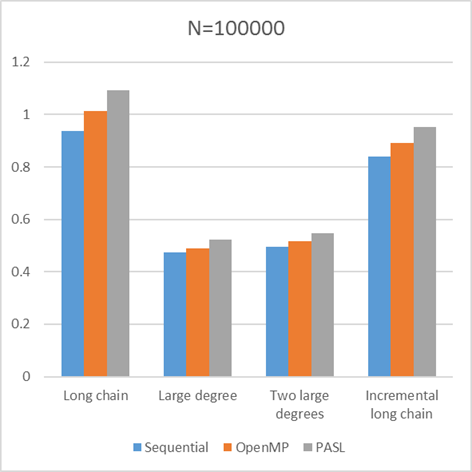
\includegraphics[width=0.45\textwidth]{tests/results-1-b.png} }}\\
\scalebox{0.65}{
\subfigure{      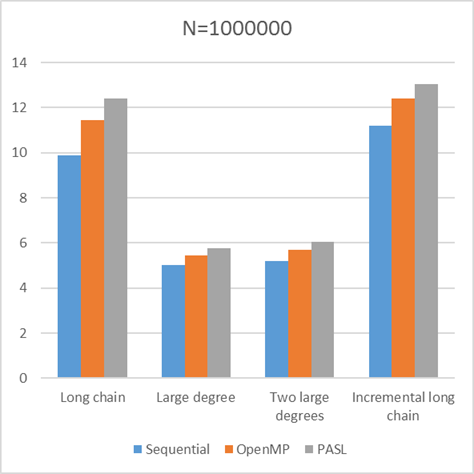
\includegraphics[width=0.45\textwidth]{tests/results-1-c.png} }
\subfigure{      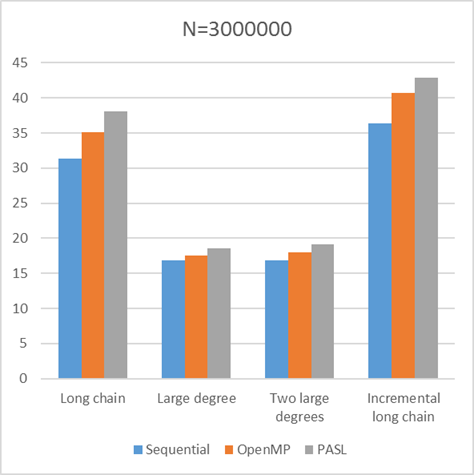
\includegraphics[width=0.45\textwidth]{tests/results-1-d.png} }}
\end{figure}
\end{center}
\end{frame}

\begin{frame}[shrink]{Результаты экспериментов: два ядра}

\begin{table}[!ht]
\centering
\scalebox{0.75}{
\begin{tabular}{|l|l|l|l|l|}\hline
Sequential	& $n=10000$ & $n=100000$ & $n=1000000$ & $n=3000000$ \\\hline
1 long chain & 0.063533	& 0.936087 & 9.8946 & 31.3906 \\\hline
2 large degree & 0.031963 & 0.473844 & 5.04014 & 16.8301 \\\hline
3 two large degrees & 0.03333 & 0.495401 & 5.19158 & 16.8656 \\\hline
4 incremental long chain & 0.068615 & 0.840358 & 11.1828 & 36.3289 \\\hline
\end{tabular}}
\end{table}

\begin{table}[!ht]
\centering
\scalebox{0.75}{
\begin{tabular}{|l|l|l|l|l|}\hline
OpenMP	& $n=10000$ & $n=100000$ & $n=1000000$ & $n=3000000$ \\\hline
1 long chain & 0.081845 & 1.10473 & 11.6696 & 35.7506 \\\hline
2 large degree & 0.04275 & 0.510112 & 5.47687 & 18.0637 \\\hline
3 two large degrees & 0.044991 & 0.529194 & 5.59677 & 17.8966 \\\hline
4 incremental long chain & 0.11298 & 1.00143 & 12.9886 & 41.9446 \\\hline
\end{tabular}}
\end{table}

\begin{table}[!ht]
\centering
\scalebox{0.75}{
\begin{tabular}{|l|l|l|l|l|}\hline

PASL	& $n=10000$ & $n=100000$ & $n=1000000$ & $n=3000000$ \\\hline
1 long chain & 0.141362	& 1.61106 & 15.5824 & 47.6541 \\\hline
2 large degree & 0.077958 & 0.859135 & 8.91695 & 28.6172 \\\hline
3 two large degrees & 0.078529 & 0.88774 & 8.77827 & 29.134 \\\hline
4 incremental long chain & 0.155524 & 1.90973 & 18.7348 & 58.2101 \\\hline
\end{tabular}}
\end{table}
\end{frame}

\begin{frame}[shrink]{Результаты экспериментов: два ядра}
\begin{center}
\begin{figure}
\centering
\scalebox{0.65}{
\subfigure{      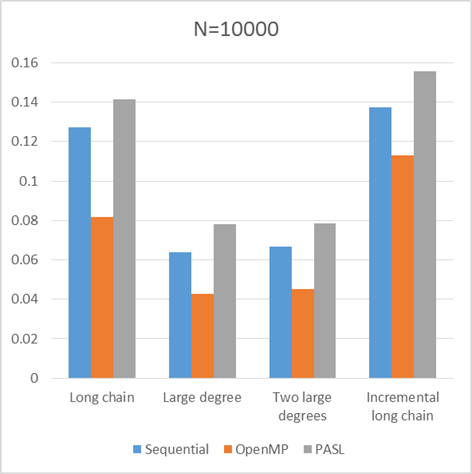
\includegraphics[width=0.45\textwidth]{tests/results-2-a.png} }
\subfigure{      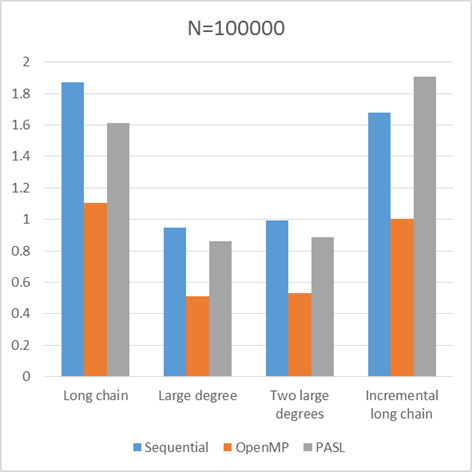
\includegraphics[width=0.45\textwidth]{tests/results-2-b.png} }}\\
\scalebox{0.65}{
\subfigure{      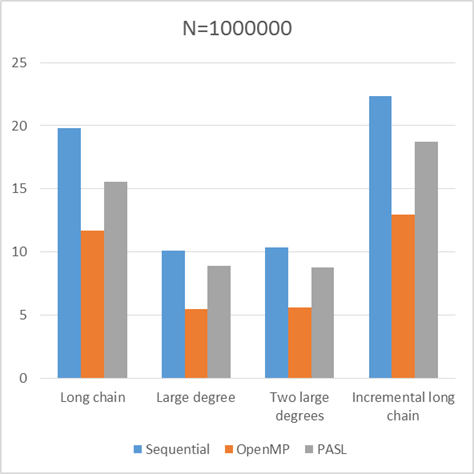
\includegraphics[width=0.45\textwidth]{tests/results-2-c.png} }
\subfigure{      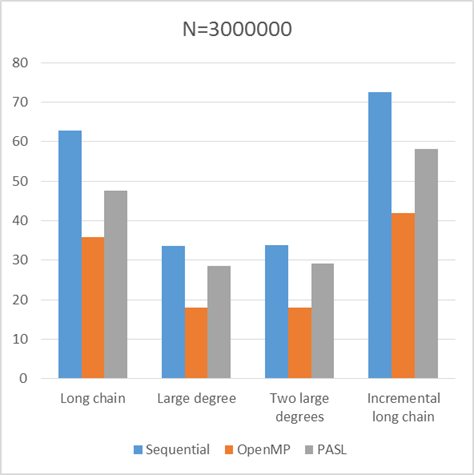
\includegraphics[width=0.45\textwidth]{tests/results-2-d.png} }}
\end{figure}
\end{center}
\end{frame}
\begin{frame}[shrink]{Результаты экспериментов: четыре ядра}

\begin{table}[!ht]
\centering
\scalebox{0.75}{
\begin{tabular}{|l|l|l|l|l|}\hline
Sequential	& $n=10000$ & $n=100000$ & $n=1000000$ & $n=3000000$ \\\hline
1 long chain & 0.063533	& 0.936087 & 9.8946 & 31.3906 \\\hline
2 large degree & 0.031963 & 0.473844 & 5.04014 & 16.8301 \\\hline
3 two large degrees & 0.03333 & 0.495401 & 5.19158 & 16.8656 \\\hline
4 incremental long chain & 0.068615 & 0.840358 & 11.1828 & 36.3289 \\\hline
\end{tabular}}
\end{table}

\begin{table}[!ht]
\centering
\scalebox{0.75}{
\begin{tabular}{|l|l|l|l|l|}\hline
OpenMP	& $n=10000$ & $n=100000$ & $n=1000000$ & $n=3000000$ \\\hline
1 long chain & 0.089218 & 1.22818 & 13.169 & 40.9343 \\\hline
2 large degree & 0.07859 & 0.553611 & 5.78005 & 18.871 \\\hline
3 two large degrees & 0.047683 & 0.583647 & 5.94402 & 18.8319 \\\hline
4 incremental long chain & 0.159757 & 1.12068 & 14.4973 & 47.2622 \\\hline
\end{tabular}}
\end{table}

\begin{table}[!ht]
\centering
\scalebox{0.75}{
\begin{tabular}{|l|l|l|l|l|}\hline
PASL	& $n=10000$ & $n=100000$ & $n=1000000$ & $n=3000000$ \\\hline
1 long chain & 0.28281	& 2.71137 & 22.9835 & 69.6526 \\\hline
2 large degree & 0.149832 & 1.5798 & 14.5509 & 49.3806 \\\hline
3 two large degrees & 0.162006 & 1.61922 & 14.9153 & 48.653 \\\hline
4 incremental long chain & 0.313789 & 3.73799 & 31.7739 & 93.2229 \\\hline
\end{tabular}}
\end{table}
\end{frame}

\begin{frame}[shrink]{Результаты экспериментов: четыре ядра}
\begin{center}
\begin{figure}
\centering
\scalebox{0.65}{
\subfigure{      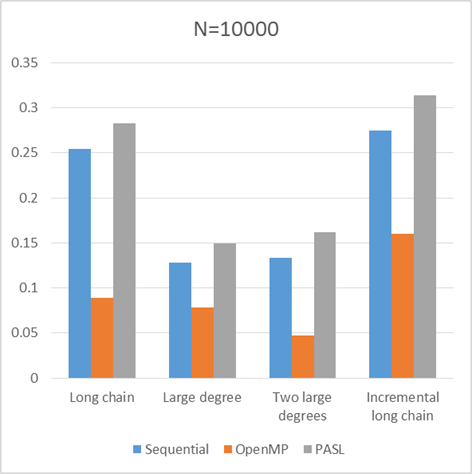
\includegraphics[width=0.45\textwidth]{tests/results-4-a.png} }
\subfigure{      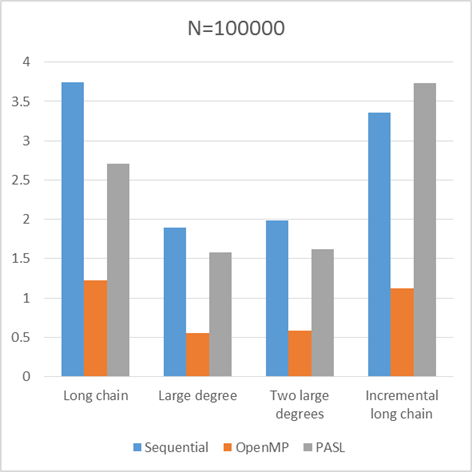
\includegraphics[width=0.45\textwidth]{tests/results-4-b.png} }}\\
\scalebox{0.65}{
\subfigure{      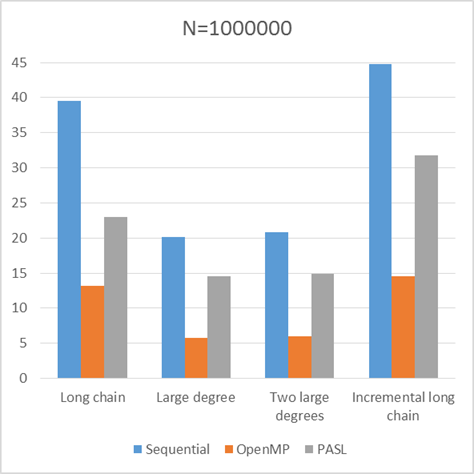
\includegraphics[width=0.45\textwidth]{tests/results-4-c.png} }
\subfigure{      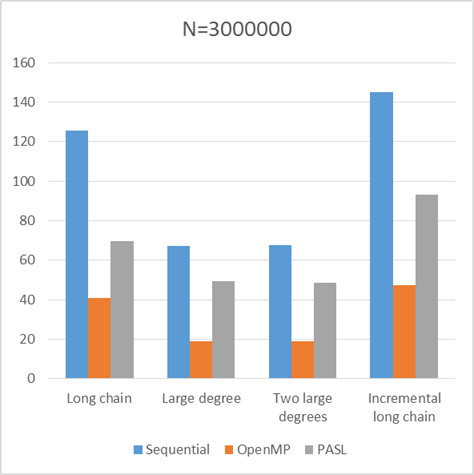
\includegraphics[width=0.45\textwidth]{tests/results-4-d.png} }}
\end{figure}
\end{center}
\end{frame}

\begin{frame}[shrink]{Результаты экспериментов: восемь ядер}

\begin{table}[!ht]
\centering
\scalebox{0.75}{
\begin{tabular}{|l|l|l|l|l|}\hline
Sequential	& $n=10000$ & $n=100000$ & $n=1000000$ & $n=3000000$ \\\hline
1 long chain & 0.063533	& 0.936087 & 9.8946 & 31.3906 \\\hline
2 large degree & 0.031963 & 0.473844 & 5.04014 & 16.8301 \\\hline
3 two large degrees & 0.03333 & 0.495401 & 5.19158 & 16.8656 \\\hline
4 incremental long chain & 0.068615 & 0.840358 & 11.1828 & 36.3289 \\\hline
\end{tabular}}
\end{table}

\begin{table}[!ht]
\centering
\scalebox{0.75}{
\begin{tabular}{|l|l|l|l|l|}\hline
OpenMP	& $n=10000$ & $n=100000$ & $n=1000000$ & $n=3000000$ \\\hline
1 long chain & 0.103436 & 1.61389 & 17.3962 & 54.0412 \\\hline
2 large degree & 0.067749 & 0.638183 & 6.74281 & 21.2547 \\\hline
3 two large degrees & 0.072668 & 0.638638 & 7.00279 & 21.7108 \\\hline
4 incremental long chain & 0.340943 & 1.39135 &	17.9712 & 58.4357 \\\hline
\end{tabular}}
\end{table}

\begin{table}[!ht]
\centering
\scalebox{0.75}{
\begin{tabular}{|l|l|l|l|l|}\hline
PASL	& $n=10000$ & $n=100000$ & $n=1000000$ & $n=3000000$ \\\hline
1 long chain & 0.563715	& 5.00583 & 39.7913 & 121.166 \\\hline
2 large degree & 0.306949 & 2.98072 & 27.0531 & 89.4415 \\\hline
3 two large degrees & 0.322895 & 3.15966 & 28.327 & 87.608 \\\hline
4 incremental long chain & 0.644581 & 7.4977 & 57.6276 & 167.604 \\\hline
\end{tabular}}
\end{table}
\end{frame}

\begin{frame}[shrink]{Сводные результаты экспериментов: OpenMP}
\begin{center}
\begin{figure}
\centering
\scalebox{0.65}{
\subfigure{      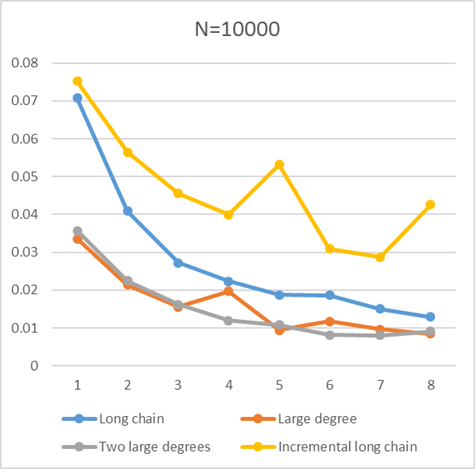
\includegraphics[width=0.45\textwidth]{tests/openmp-a.png} }
\subfigure{      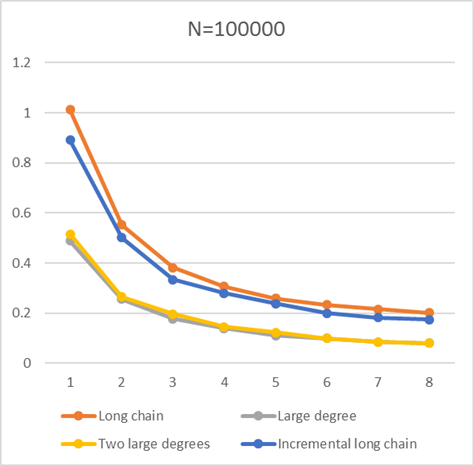
\includegraphics[width=0.45\textwidth]{tests/openmp-b.png} }}\\
\scalebox{0.65}{
\subfigure{      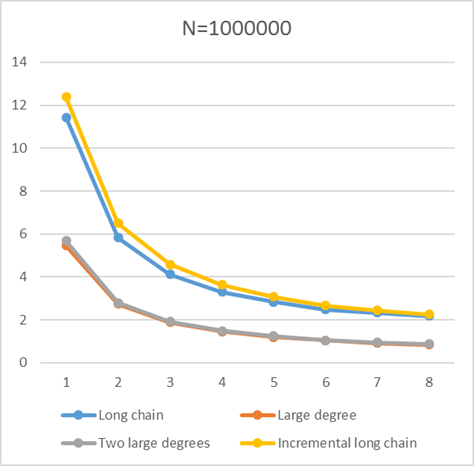
\includegraphics[width=0.45\textwidth]{tests/openmp-c.png} }
\subfigure{      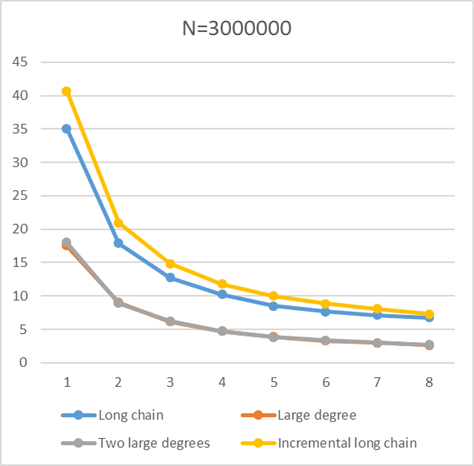
\includegraphics[width=0.45\textwidth]{tests/openmp-d.png} }}
\end{figure}
\end{center}
\end{frame}

\begin{frame}[shrink]{Сводные результаты экспериментов: PASL}
\begin{center}
\begin{figure}
\centering
\scalebox{0.65}{
\subfigure{      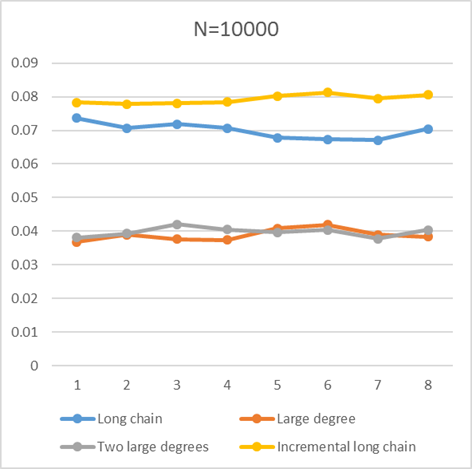
\includegraphics[width=0.45\textwidth]{tests/pasl-a.png} }
\subfigure{      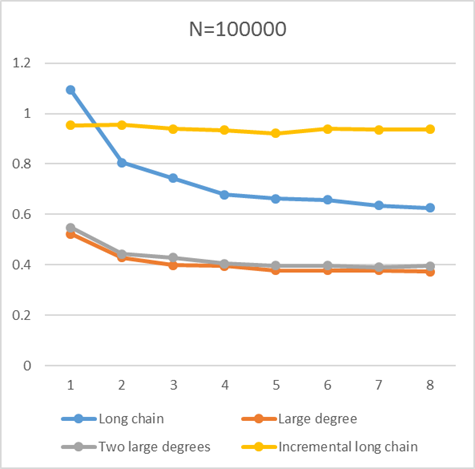
\includegraphics[width=0.45\textwidth]{tests/pasl-b.png} }}\\
\scalebox{0.65}{
\subfigure{      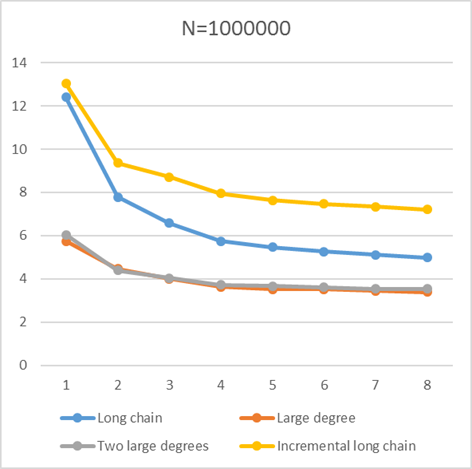
\includegraphics[width=0.45\textwidth]{tests/pasl-c.png} }
\subfigure{      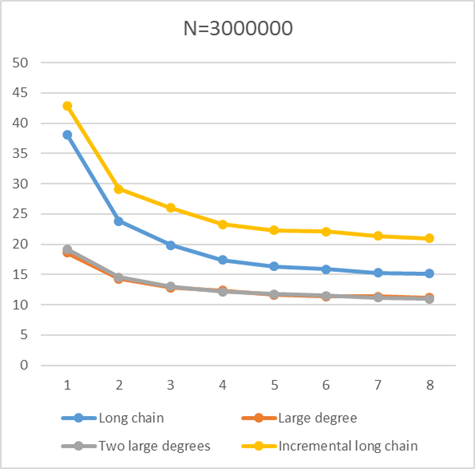
\includegraphics[width=0.45\textwidth]{tests/pasl-d.png} }}
\end{figure}
\end{center}
\end{frame}

\begin{frame}[shrink]{Заключение}
\begin{itemize}
    \item Разработан параллельный алгоритм построения и применения пакетов изменений к RC-деревьям
    \item Разработаны параллельные реализации алгоритма с использованием библиотек параллельных вычислений OpenMP и PASL
    \item Распараллеливание с использованием PASL менее эффективно для работы с RC-деревьями
\end{itemize}

\end{frame}

\begin{frame}[shrink]{Апробация работы}
\begin{itemize}
\item Публикации:\nocite{wjf-kmu, wjf-spisok}
\printbibliography 
\end{itemize}
\end{frame}
\begin{frame}[shrink]{~~~}
\begin{center}
\Huge Спасибо за внимание!
\end{center}
\end{frame}
\end{document}

